Stochastic Gradient Descent (SGD) is also employed for the machine learning process. SGD is an iterative method that is a stochastic approximation of typical gradient descent. SGD tends to achieve faster computation time of iterations at the expense of a slower convergence rate. In typical gradient descent, the gradient of the objective function is computed over the entire domain  of data points, whereas SGD takes sampled subsets of the domain and approximates the gradient over this random sample. That is, in typical gradient descent for machine learning, our problem may look like
\begin{align*}
    \text{minimize} \hspace{1em} f(x) = \frac{1}{2}\sum_{i \in D} \|N(x) - y_i \|^2\\
\end{align*}
Where $N(x)$ is the neural network approximation and $y_i$ is the measured data. The associated update step is given by
\[x_{k+1} = x_k - \alpha \nabla f(x)\]
With SGD, we restrict our attention to $i \in S \subset D$ so that the update step looks like
\[x_{k+1} = x_k - \alpha \nabla f_i(x)\]
where $\nabla f_i(x)$ is the estimated gradient of $f$ over a domain sample.
\newline\newline


A variation of SGD that was utilized was the Adam SGD method. Adam (Adaptive Moment Estimation) runs averages with exponential \say{forgetting} of both gradients and second moments of gradients. Given parameters $w^{(t)}$ and a loss function $L^{(t)}$ with $t$ indexing the current training iteration starting from 0, the Adam parameter update is given by
\begin{figure}[H]
    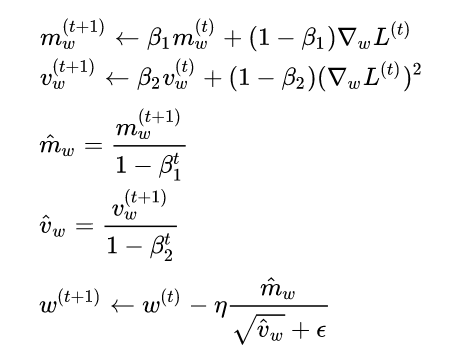
\includegraphics[scale = 1]{images/adam.png}
    \centering
    \caption{Outline of the Adams stochastic gradient descent algorithm. Taken from Wikipedia.}
\end{figure}
with $\epsilon$ small (i.e. $10^{-8})$ and $\beta_1$ (i.e. 0.9) and $\beta_2$ (i.e. 0.999) are called the forgetting factors for the gradients and second moments of the gradients. The square root and squaring operations are done elementwise. 